\documentclass[11pt,letterpaper]{article}
\usepackage[lmargin=1in,rmargin=1in,tmargin=1in,bmargin=1in]{geometry}
\usepackage{../style/homework}
\usepackage{../style/commands}
\setbool{quotetype}{true} % True: Side; False: Under
\setbool{hideans}{false} % Student: True; Instructor: False

% -------------------
% Content
% -------------------
\begin{document}

\homework{9: Due 04/14}{Poetry is as precise a thing as geometry.}{Gustave Flaubert}

% Problem 1
\problem{10} Showing all your work, complete the following:
	\begin{enumerate}[(a)]
	\item Find the interior and exterior angles for a regular polygon with 22 sides. 
	\item Find the smallest angle between the hour and minute hand of an analog clock at 10:20. 
	\item Find $x$ in the diagram below:
		\[
		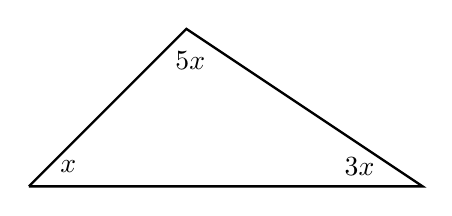
\begin{tikzpicture}
		\draw[line width=0.03cm] (0,0) -- (2,2) -- (5,0) -- (0,0);
		\node at (0.5,0.25) {$x$};
		\node at (2.05,1.6) {$5x$};
		\node at (4.2,0.25) {$3x$};
		\end{tikzpicture}
		\]
	\end{enumerate} \pspace

\sol 
\begin{enumerate}[(a)]
\item The sum of the interior angles of an $n$-gon is $(n - 2)180^\circ$. We have $n= 22$ so that the sum of the interior angles is $(22 - 2) 180^\circ= 20 \cdot 180^\circ= 3600^\circ$. Because the polygon is regular, all the angles are congruent. But then each interior angle has measure $\frac{3600^\circ}{22}= 163.636^\circ$. The sum of the exterior angles of a regular $n$-gon is $360^\circ$. Because the polygon is regular, each exterior angle is congruent. But then each exterior angle has measure $\frac{360^\circ}{22}= 16.364^\circ$. \pspace

\item We measure the angle from the 12, i.e. from the vertical. Because the minute hand revolves once around the clock in 60 minutes, the minute hand moves $\frac{360^\circ}{60}= 6^\circ$ per minute. We know that every hour, the hour hand revolves $\frac{1}{12}$ of the way around the circle. But then the hour hand moves $\frac{1}{12} \cdot 360^\circ= 30^\circ$ every hour. But the hour hand also moves because the minute hand moves. We know every 60 minutes, the hour hand moves $30^\circ$. But then the hour hand moves $\frac{30^\circ}{60}= 0.5^\circ$ every minute. After 10~hours, the hour hand has moved $10 \cdot 30^\circ= 300^\circ$. Then after another 20~minutes, the hour hand has moved an additional $20 \cdot 0.5^\circ= 10^\circ$. Therefore, the hour hand makes an angle of $300^\circ + 10^\circ= 310^\circ$ from the vertical. The minute hand starts at the vertical at 10:00. After 20 minutes, the minute hand has moved $20 \cdot 6^\circ= 120^\circ$. But then the minute hand makes a $120^\circ$ with the vertical. Therefore, the angle between then is $310^\circ - 120^\circ= 190^\circ$. \pspace

\item The sum of the angles inside a triangle is $180^\circ$. But then we know $x + 5x + 3x= 180^\circ$. But then\dots
	\[
	\begin{aligned}
	x + 5x + 3x&= 180^\circ \\[0.3cm]
	9x&= 180^\circ \\[0.3cm]
	\dfrac{9x}{9}&= \dfrac{180^\circ}{9} \\[0.3cm]
	x&= 20^\circ
	\end{aligned}
	\]
\end{enumerate}



\newpage



% Problem 2
\problem{10} Assuming that the two horizontal lines are parallel, find all the angles labeled in the diagram below:
	\[
	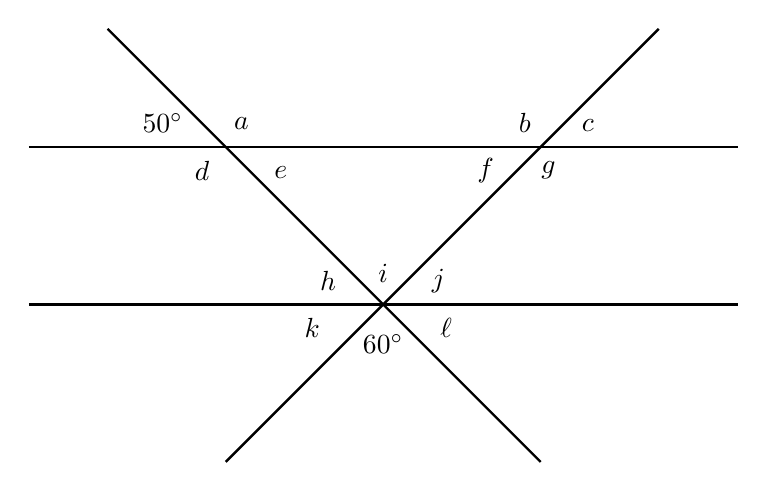
\begin{tikzpicture}
	\draw[line width=0.03cm] (-4.5,2) -- (4.5,2);
	\draw[line width=0.03cm] (-4.5,0) -- (4.5,0);
	\draw[line width=0.03cm] (-2,-2) -- (3.5,3.5);
	\draw[line width=0.03cm] (-3.5,3.5) -- (2,-2);
	\node at (-2.8,2.3) {$50^\circ$};
	\node at (-1.8,2.3) {$a$};
	\node at (1.8,2.3) {$b$};
	\node at (2.6,2.27) {$c$};
	\node at (-2.3,1.7) {$d$};
	\node at (-1.3,1.67) {$e$};
	\node at (1.3,1.7) {$f$};
	\node at (2.1,1.7) {$g$};
	\node at (-0.7,0.3) {$h$};
	\node at (0,0.4) {$i$};
	\node at (0.7,0.3) {$j$};
	\node at (-0.9,-0.3) {$k$};
	\node at (0,-0.5) {$60^\circ$};
	\node at (0.8,-0.3) {$\ell$};
	\end{tikzpicture}
	\] \pspace

\sol Because $50^\circ$ and $a$ are supplementary, we know that $50^\circ + a= 180^\circ$. But then $a= 130^\circ$. But because $50^\circ$ and $e$ as well as $a$ and $d$ are vertical angles, each pair is congruent. But then $a= 130^\circ= d$ and $e= 50^\circ$. But because the lines are parallel, we know that the alternate interior angles are congruent. But then $e$ and $h$ are congruent. This shows that $e= 50^\circ= h$. But angle $i$ and $60^\circ$ are vertical angles. This shows that $i= 60^\circ$. But because $h$, $i$, and $j$ are supplementary, we know that $h + i + j= 180^\circ$. Then $50^\circ + 60^\circ + j= 180^\circ$ so that $j= 70^\circ$. Because $h$ and $\ell$ as well as $k$ and $j$ are vertical angles, each pair is congruent. But then we know that $h= 50^\circ= \ell$ and $j= 70^\circ= k$. But because the lines are parallel, the alternate interior angles are congruent. This shows that $j$ and $f$ are congruent. But then $j= 70^\circ= f$. Now $f$ and $g$ are supplementary so that $f + g= 180^\circ$. But then $70^\circ + g= 180^\circ$ so that $g= 110^\circ$. Finally, because $b$ and $g$ as well as $f$ and $c$ are vertical angles, each pair is congruent. This shows that $f= 70^\circ= c$ and $g= 110^\circ= b$. Therefore, we have\dots \pspace
	\[
	\begin{aligned}
	a&= 130^\circ &\qquad g&= 110^\circ \\[0.3cm]
	b&= 110^\circ & h&= 50^\circ \\[0.3cm]
	c&= 70^\circ & i&= 60^\circ \\[0.3cm]
	d&= 130^\circ & j&= 70^\circ \\[0.3cm]
	e&= 50^\circ & k&= 70^\circ \\[0.3cm]
	f&= 70^\circ & \ell&= 50^\circ
	\end{aligned}
	\]



\newpage



% Problem 3
\problem{10} A student claims that all rectangles are always squares, rhombuses are never squares, and trapezoids are sometimes squares. Which, if any, of these statements are correct and which are incorrect? How would you help this student understand these concepts? \pspace

\sol While squares are always rectangles, rectangles need not be squares. Furthermore, while not all rhombuses are square, squares always always rhombuses. So some rhombuses are squares. Trapezoids sometimes are square.\footnote{This assumes that the definition of a trapezoid is a quadrilateral with at least one pair of parallel sides. Some define a trapezoid to be a quadrilateral with \textit{exactly} one pair of parallel sides. Using this definition, trapezoids cannot be rhombuses, rectangles, or squares.} Therefore, the student's first two statements are incorrect and the last is correct. The student seems to have the implication directions reversed. A good exercise for the student would be to draw an example and non-example of each parallelogram, e.g. a rectangle that is square and a rectangle that is not a square. 


\end{document}